% MTE 481 - Preliminary Design Presentation
% Group 2
%
% A neat PDF slideshow.

%%%%%%%%%%%%
% Preamble %
%%%%%%%%%%%%
\documentclass{beamer}
\mode<presentation>

\usepackage{graphicx}

\title{MTE 481 - Design Project}
\subtitle{Object Avoidance and Navigation for Powered Wheelchairs}
\author{Iain Peet \and Rowan Head-Marsden \and Jordan Valentin}

%%%%%%%%
% Body %
%%%%%%%%
\begin{document}

\begin{frame}
  \titlepage
\end{frame}

\begin{frame}
  \frametitle{Introduction}
  \begin{figure}
    \centering
    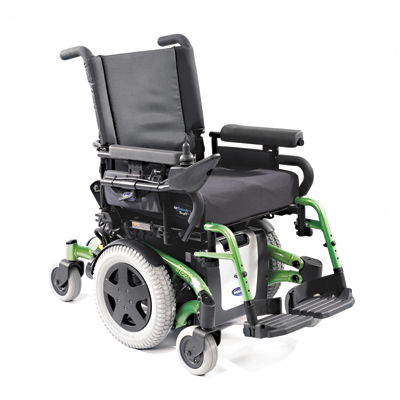
\includegraphics[width=6cm]{wheelchair.jpg} 
  \end{figure}
\end{frame}

\begin{frame}
  \frametitle{Need Statement}
  Powered wheelchairs can improve the mobility of the physically handicapped, but 
  alertness and control are required for safe operation.
  Additional assistive technology is needed in order to afford the same benefits
  to the more severely disabled.
\end{frame}

\begin{frame}
  \frametitle{Potential Impact}
  \begin{itemize}
    \item Risk of collisions between powered wheelchairs and patients is a serious concern. \\
    \item Significant quantity of patients denied powered wheelchairs due to relatively minor impairments. \\
  \end{itemize}
\end{frame}

\begin{frame}
  \frametitle{Objectives and Constraints}
  \begin{itemize}
    \item Risk of human harm must be made negligible. \\
    \item Must be tolerant of user error. \\
    \item Should tolerate a wide variety of operating environments. \\
    \item Cost should be minimized. \\
    \item Electrical power usage should be minimized. \\
    \item Should be physically robust. \\
  \end{itemize}
\end{frame}

\begin{frame}
  \frametitle{Criteria}
\end{frame}

\begin{frame}
  \frametitle{Potential Solutions}
\end{frame}

\begin{frame}
  \frametitle{Potential Solution 1 Detail}
\end{frame}

\begin{frame}
  \frametitle{Potential Solution 2 Detail}
\end{frame}

\begin{frame}
  \frametitle{Patent Search Results}
\end{frame}

\end{document}
